%%%%%%%%%%%%%%%%%%%%%%%%%%%%%%%%%%%%%%%%%%%%%%%%%%%%%%%%%%%%%%%%%%%%%%
% Problem statement
\begin{statement}[
  problempoints=30,
  timelimit=1 sekunda,
  memorylimit=512 MiB,
]{Hajduk}

\setlength\intextsep{-0.1cm}
\begin{wrapfigure}[5]{r}{0.26\textwidth}
\centering
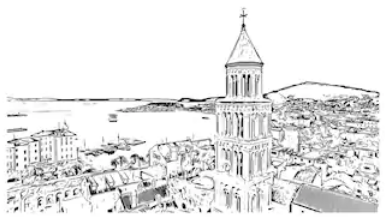
\includegraphics[width=0.26\textwidth]{img/split.png}
\end{wrapfigure}

Badnjak je. U Splitu pred katedralom sv. Duje okupilo se mnoštvo ljudi čekajući
polnoćku.

Čuje se \textit{Tiha noć} i miriše na fritule, a $N$ članova navijačke skupine
\textit{Torcida} razbija tišinu i glasa za novog trenera Hajduka. Trenera biraju
između $K$ ponuđenih nogometnih stručnjaka označenih prirodnim brojevima od $1$
do $K$, a pobjedu odnosi onaj trener koji dobije \textbf{barem polovicu
glasova}.  U slučaju da dva trenera dobiju po pola glasova, pobjedu odnosi
onaj s manjom oznakom.  Marin iz prikrajka prati glasanje i zapisuje za koga
je glasao koji navijač.  Na kraju glasanja, želi saznati hoće li njegov
prijatelj, trener s oznakom $1$, dočekati Božić na klupi Hajduka.

Pomozite Marinu odgovoriti na pitanje.


%%%%%%%%%%%%%%%%%%%%%%%%%%%%%%%%%%%%%%%%%%%%%%%%%%%%%%%%%%%%%%%%%%%%%%
% Input
\subsection*{Ulazni podaci}
U prvom je retku prirodan broj $N$ $(1 \le N \le 100)$ iz teksta zadatka.

U drugom je retku prirodan broj $K$ $(1 \le K \le 100)$ iz teksta zadatka.

U sljedećih se $N$ redaka nalazi po jedan prirodan broj, oznaka trenera za kojeg
je glasao $i$-ti navijač.

%%%%%%%%%%%%%%%%%%%%%%%%%%%%%%%%%%%%%%%%%%%%%%%%%%%%%%%%%%%%%%%%%%%%%%
% Output
\subsection*{Izlazni podaci}
U jedini redak ispišite \texttt{"DA"} (bez navodnika) ako će trener s oznakom
$1$ preuzeti klupu Hajduka, odnosno \texttt{"NE"} (bez navodnika) ako neće.

%%%%%%%%%%%%%%%%%%%%%%%%%%%%%%%%%%%%%%%%%%%%%%%%%%%%%%%%%%%%%%%%%%%%%%
% Scoring
 \subsection*{Bodovanje}
U test podacima ukupno vrijednima $10$ bodova vrijedi $N=K=2$.\\
U test podacima vrijednima dodatnih $10$ bodova vrijedi $N=K=3$.

%%%%%%%%%%%%%%%%%%%%%%%%%%%%%%%%%%%%%%%%%%%%%%%%%%%%%%%%%%%%%%%%%%%%%%
% Examples
\subsection*{Probni primjeri}
\begin{tabularx}{\textwidth}{X'X'X}
\sampleinputs{test/hajduk.dummy.in.1}{test/hajduk.dummy.out.1} &
\sampleinputs{test/hajduk.dummy.in.2}{test/hajduk.dummy.out.2} &
\sampleinputs{test/hajduk.dummy.in.3}{test/hajduk.dummy.out.3}
\end{tabularx}

\textbf{Pojašnjenje trećeg probnog primjera:}
Trener s oznakom $1$ je dobio jednako glasova kao i treneri s oznakama $2$ i
$3$, ali nije sakupio barem polovicu glasova.

%%%%%%%%%%%%%%%%%%%%%%%%%%%%%%%%%%%%%%%%%%%%%%%%%%%%%%%%%%%%%%%%%%%%%%
% We're done
\end{statement}

%%% Local Variables:
%%% mode: latex
%%% mode: flyspell
%%% ispell-local-dictionary: "croatian"
%%% TeX-master: "../hio.tex"
%%% End:
